\section*{CHAPTER 1: THEORETICAL BACKGROUND}
\addcontentsline{toc}{section}{\numberline{}CHAPTER 1:THEORETICAL BACKGROUND}
\setcounter{section}{1}
\setcounter{subsection}{0}
\setcounter{figure}{0}
\setcounter{table}{0}

This chapter focuses on providing the theoretical foundations and background knowledge necessary to understand the concepts and methodologies discussed in the subsequent chapters of this project.

\subsection{Single-carrier modulation technique}
% In Single-carrier modulation, only one Radio Frequency (RF) carrier is used to carry the information.
In Single-carrier modulation, the signal is transmitted across the entire bandwidth $B$ \cite{OFDM2006}, meaning that the system's sampling frequency is equal to the bandwidth, and each signal has a length of:
\begin{equation}
    T_{SC} = \frac{1}{B}
    \label{eq:single-carrier}
\end{equation}

In Equation \ref{eq:single-carrier}, $T_{SC}$ is the duration of a signal sample, measured in seconds (s); $B$ is the bandwidth of the system, measured in Hertz (Hz). In broadband wireless communication, the radio channel is usually frequency selective, and the sampling frequency is very high, resulting in the sample duration $T_{SC}$ being very small. Therefore single-carrier modulation technique has several disadvantages:

\begin{itemize}
    \item Large Inter-symbol interference (ISI): The symbol period must be much greater than the delay time in order to avoid ISI.
    \item Low data rate: since data rate is inversely proportional to symbol period, having long symbol periods means low data rate and communication inefficiency.
\end{itemize}

To address these disadvantages, a multi-carrier system, such as FDM is developed.

\subsection{Multi-carrier modulation technique}

Frequency division multiplexing (FDM) is a multi-carrier modulation technique by which the total bandwidth available in a communication medium is divided into a series of non-overlapping frequency bands, each of which is used to carry a separate signal \cite{b2}.
An overall high data rate can be achieved by placing carriers closely in the spectrum. However, inter-carrier interference (ICI) will occur due to a lack of spacing to separate the carriers. To avoid inter-carrier interference, guard bands will need to be placed in between any adjacent carriers, which results in a lowered data rate.

\subsection{OFDM technique}

\subsubsection{OFDM Definition}

Orthogonal Frequency Division Multiplexing (OFDM) is a special case of the Frequency Division Multiplexing (FDM) technique \cite{OFDM2010}.
% In digital communications, information is expressed in the form of bits. The term symbol refers to a collection, in various sizes, of bits \cite{Litwin2001}.
OFDM data are generated by taking symbols in the spectral space using M-PSK, QAM, etc, and convert the spectra to time domain by taking the Inverse Discrete Fourier Transform (IDFT). Since Inverse Fast Fourier Transform (IFFT) is more cost effective to implement, it is usually used instead \cite{b3}. Once the OFDM data are modulated to time signal, all carriers transmit in parallel to fully occupy the available frequency bandwidth. During modulation, OFDM symbols are typically divided into frames, so that the data will be modulated frame by frame in order for the received signal be in sync with the receiver. Long symbol periods diminish the probability of having inter-symbol interference, but could not eliminate it. To make ISI nearly eliminated, a cyclic prefix (CP) is added to each symbol period. An exact copy of a fraction of the cycle, typically 25\% of the cycle, taken from the end is added to the front. This allows the demodulator to capture the symbol period with an uncertainty of up to the length of a cyclic extension and still obtain the correct information for the entire symbol period.

\begin{figure}[ht]
    \centering
    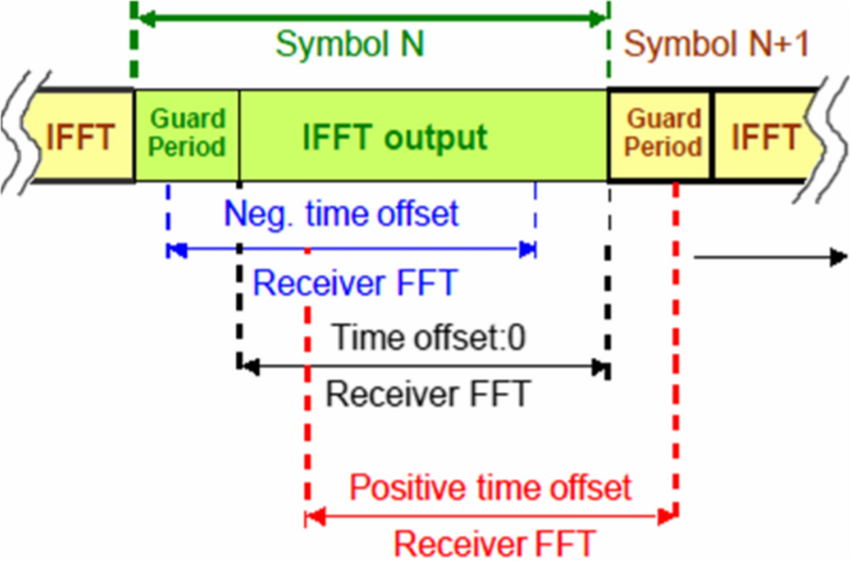
\includegraphics[width=0.5\textwidth]{Figures/Cyclic-extension-tolerance}
    \caption{Cyclic prefix tolerance}
    \label{Cyclic-extension-tolerance}
\end{figure}

As shown in Figure \ref{Cyclic-extension-tolerance}, a guard period, another name for the cyclic extension, is the amount of uncertainty allowed for the receiver to capture the starting point of a symbol period, such that the result of FFT still has the correct information. In Figure 2, a comparison between a precisely detected symbol period and a delayed detection illustrates the effectiveness of the cyclic extension.

\begin{figure}[ht]
    \centering
    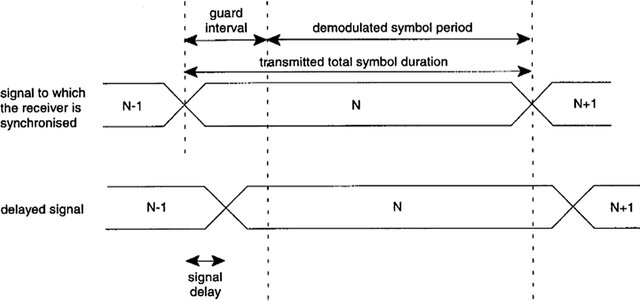
\includegraphics[width=\textwidth]{Figures/Effectiveness-of-cyclic-extension}
    \caption{Effectiveness-of-cyclic-extension}
    \label{Effectiveness-of-cyclic-extension}
\end{figure}
% \subsubsection{Complexity}

% The number of carriers in an OFDM system is not only limited by the available spectral bandwidth, but also by the IFFT size, which is determined by the complexity of the system. The more complex (also more costly) the OFDM system is, the higher IFFT size it has; thus a higher number of carriers can be used, and higher data transmission rate achieved.
% % The choice of M-PSK modulation varies the data rate and Bit Error Rate (BER). The higher order of PSK leads to larger symbol size, thus less number of symbols needed to be transmitted, and higher data rate is achieved. But this results in a higher BER since the range of 0-360 degrees of phases will be divided into more sub-regions, and the smaller size of sub-regions is required, thereby received phases have higher chances to be decoded incorrectly.
% OFDM signals have high peak-to-average ratio, therefore it has a relatively high tolerance of peak power clipping due to transmission limitations.

\subsubsection{Orthogonality}

The key to OFDM is maintaining orthogonality of the carriers. If the integral of the product of two signals is zero over a time period, then these two signals are said to be orthogonal to each other. Two sinusoids with frequencies that are integer multiples of a common frequency can satisfy this criterion. Therefore, orthogonality is defined by :

\begin{equation}\label{eq1}
    \int_{0}^{T} cos(2 \pi n f_o t) cos(2 \pi m f_o t) \,dt = 0 \quad (n \neq m)
\end{equation}

Where $n$ and $m$ are two unequal integers; $f_o$ is the fundamental frequency; $T$ is the period over which the integration is taken. For OFDM, $T$ is one symbol period and $f_o$ set to to $\frac{1}{T}$ for optimal effectiveness.

\subsubsection{Advantages and Disadvantages}

Upgrading and optimizing algorithms, OFDM systems provide highly advantageous features for wireless transmission and transceiver system design:

\begin{itemize}
    \item Since the symbol duration is inversely proportional to the symbol rate, each subcarrier has relatively long symbols. Long symbols are robust against multipath fading, as it occurs in wireless systems.
    \item When a carrier is in a deep fade due to frequency-selectivity of the channel (i.e. the received energy on this carrier is very low), only the data on this subcarrier is lost, instead of the whole stream.
    \item Multicarrier systems allow easy multi-user resource sharing by allocating different subcarriers to different users.
\end{itemize}
However, OFDM technology also has its drawbacks that need careful consideration and practical research for designing a system suitable for specific purposes:
\begin{itemize}
    \item Uneven Amplitude Envelope: The amplitude envelope of the signal is uneven, causing nonlinear distortion in power amplifiers at the transmitter and receiver.
    \item Guard Interval Impact on Transmission Efficiency: While the guard interval is used to eliminate ISI, it also reduces transmission efficiency due to wasting power on transmitting useless signals.
    \item Orthogonality Conditions between Subcarriers: The requirement for orthogonality between subcarriers makes the system susceptible to the effects of Doppler, frequency offset, and time offset due to synchronization errors.
\end{itemize}
These challenges require careful consideration and research to optimize the performance of the OFDM system under real-world conditions and ensure that the drawbacks do not significantly affect transmission quality

\subsection{Conclusion}

In conclusion, chapter 1 has provided a comprehensive theoretical background necessary for understanding the concepts and methodologies explored in this project, such as: FDM, OFDM, FFT. Now we move on to the next chapter, where we're going to survey some of the existing paper recognition methods and our own proposed methods.
